\documentclass[mathserif, aspectratio=169]{beamer}
\usetheme{odenpecos}
\setbeamertemplate{itemize/enumerate body begin}{\fontsize{8.8}{9}\selectfont}
\setbeamertemplate{itemize/enumerate subbody begin}{\fontsize{7.5}{8}\selectfont}
\setbeamertemplate{itemize/enumerate subsubbody begin}{\fontsize{7.5}{8}\selectfont}

% default search path for figures
\graphicspath{{./shared_figures/}{./figures/}}

\newcommand{\zapspace}{\topsep=0pt\partopsep=0pt\itemsep=0pt\parskip=0pt}

\usepackage{multicol}
\usepackage{pict2e}
\usepackage{esdiff}
\usepackage{multimedia}
\usepackage{verbatim}
\usepackage{mhchem}

\usepackage[percent]{overpic}
\usepackage[absolute,overlay]{textpos}
\newcommand{\overbar}[1]{\mkern 1.5mu\overline{\mkern-1.5mu#1\mkern-1.5mu}\mkern 1.5mu}
\newcommand{\pp}[2]{\frac{\partial #1}{\partial #2}}
\newcommand{\dd}[2]{\frac{d #1}{d #2}}
\newcommand{\DD}[2]{\frac{D #1}{D #2}}
\newcommand{\mm}{\mathbf{minmod}}
\def\etal{{\it et al~}}
\newcommand{\be}{\begin{eqnarray}}
	\newcommand{\ee}{\end{eqnarray}}
\newcommand{\mbb}[1]{\mathbb{#1}} % math blackboard bold
\newcommand{\mcal}[1]{\mathcal{#1}} % math blackboard bold
\newcommand{\mbf}[1]{\mathbf{#1}} % math bold face (for vectors)
\newcommand{\sbf}[1]{\boldsymbol{#1}} % bold face for symbols
\newcommand{\jump}[1]{\llbracket #1 \rrbracket} % jump operator
\newcommand{\avg}[1]{\langle #1 \rangle} % average operator
\newcommand{\rarrow}{\rightarrow}
\newcommand{\Rarrow}{\Rightarrow}
\newcommand{\LRarrow}{\Leftrightarrow}
\newcommand{\vvvert}{|\kern-1pt|\kern-1pt|}
\newcommand{\enorm}[1]{\vvvert #1 \vvvert}
\newcommand{\nutil}{\tilde{\nu}}
\newcommand{\Var}{\mathrm{Var}}
\newcommand{\Cov}{\mathrm{Cov}}


\definecolor{MyDarkGreen}{rgb}{0,0.45,0.08}
\newcommand{\myred}[1]{{\color{red} #1}}
\newcommand{\myblue}[1]{{\color{blue} #1}}
\newcommand{\mygreen}[1]{{\color{MyDarkGreen} #1}}

\newcommand{\sa}{\nu_{\mathrm{sa}}}
\newcommand{\tep}{\tilde{\epsilon}}
\newcommand{\Ssd}{\mathcal{S}} % source term due to slow derivative
\newcommand{\ud}{\,\mathrm{d}}

\newcommand{\Mach}[1]{\ensuremath{\mbox{Ma}_{#1}}}
\newcommand{\Reynolds}{\ensuremath{\mathit{Re}}}
\newcommand{\DensityRat}{\ensuremath{\mathit{DR}}}
\newcommand{\BlowRat}{\ensuremath{\mbox{BR}}}
\newcommand{\VelRat}{\ensuremath{\mathit{VR}}}
\newcommand{\Tau}{\ensuremath{\mathrm{T}}}

\newcommand{\wall}     {\ensuremath{\mathrm{w}}}   % wall subindex
\newcommand{\awall}    {\ensuremath{\mathrm{aw}}}  % adiabatic wall subindex

\newcommand{\commentout}[1]{}

\newcommand{\vect}[1]{\boldsymbol{#1}}
\usepackage{mleftright}
\newcommand{\of}[1]{\mleft( #1 \mright)}
\newcommand{\vth}{v_{\textrm{th}}}
\newcommand{\reals}{\mathbb{R}}
\newcommand{\myint}[2]{\int\limits_{#1}^{#2}}
\newcommand{\norm}[1]{\left\lVert#1\right\rVert}


\DeclareMathOperator{\variance}{Var}

\begin{document}
	% disable nav
	\setbeamertemplate{navigation symbols}{}

	\begin{frame}[plain,t]{}
	\makeatletter
	%\vspace*{0.85cm}
	%\vspace*{0.65cm}
	\includegraphics[height=0.9in,trim=50 40 40 0, clip]{PMSc_159_university_formal_horizontal.pdf} \newline
	%\vspace*{0.3cm}
	\begin{columns}[T,onlytextwidth]
	\column{.8\textwidth}
	{\bf \color{burntorange} \fontfamily{bch}\selectfont 
	% -- Set talk title here
		Solving the Boltzmann equation for electron kinetics using Petrov-Galerkin approach
	% --
	}
	\end{columns}
	\vspace*{.15cm}
	\rule{.8\textwidth}{0.6pt} \newline
	
	\vspace*{0.05cm}
	\setstretch{0.65}
	{\fontfamily{phv}\selectfont
	 { \scriptsize
	   % -- define presenter, authors here
	   Milinda Fernando, Daniil Bochkov, Todd Oliver, George Biros, ...\newline
	   % --
	 }
	 {\color{burntorange} \tiny
	   % -- define role, meeting event, location, etc
	   All in hands meeting $\cdot$ December, 2021 $\cdot$ Austin, TX
	   % --
	 }
	}
	
	\vspace*{1cm}
	%\includegraphics[height=0.3in]{figures/pecos_orange1.png}
	\begin{columns}
	\begin{column}{0.8\linewidth}
	\includegraphics[height=0.5in]{oden_pecos_2020_wordmark.png}\\
	{\scriptsize \url{https://pecos.oden.utexas.edu}}
	\end{column}
	
	\begin{column}{0.2\linewidth}
	\includegraphics[height=0.6in]{psaap3-logo.png}
	\end{column}
	\end{columns}
	
	\end{frame}
	%===============================================================================
	%===============================================================================
	\begin{frame}
		\frametitle{Boltzmann equation}
		%
		\begin{itemize}
			%Electron density function $f = f(\vect{x}, \vect{v}, t)$ defines transport and kinetic properties
			% Distribution function of electrons defines transport and reaction properties
			% \\
			% $\rightarrow$ Need to couple plasma model with electron kinetics (Y3)
			\item Evolution of species distribution function $f = f(\vect{x}, \vect{v}, t)$ obeys the \textbf{Boltzmann equation}
			\small
			\begin{align*}
				\partial_t f + \vect{v}\cdot \nabla_{\vect{x}} f  - \vect{E} \cdot \nabla_{\vect{v }}f = \sum_{a} C_a(f) 
			\end{align*}
			where, $C_a$ denotes the collision term, for example, in case of $a=$ elastic collisions, with $\delta(0)$ for background distribution function, we can write,  
			\begin{align*}
				C_a(f) &= n_0\int_{S^2} |v| \underbrace{\sigma_a(v,\omega)}_{\tiny\text{\tiny scat. cross sec.}} 
				\left(|J|f(v^{pre}(v,\omega)) - f(v) \right) \ud \omega 
			\end{align*}
			\item \textbf{Challenges}: 6+1 dimensions, numerical issues,  HPC related challenges, ...
			% \item \textbf{Idea}: FEM in $\vect{x}$, spectral in $\vect{v}$
			% \item \textbf{Currently (Y1)}: spatially homogeneous case $f = f(\vect{v}, t)$ to investigate efficient velocity-space discretizations
			% \begin{align*}
			% 	\partial_t f = \sum_{a} C_a(f)
			% \end{align*}
		\end{itemize}
		Approach: Use FEM type discretization in space, and use \textcolor{orange}{spectral dirscretization} in velocity space.  
	\end{frame}

	\begin{frame}
		\frametitle{Velocity space discretization : Petrov-Galerkin approach}
		\begin{itemize}

		\item Weak formulation (currently $\bf E=0$):
		$
		\displaystyle
		\quad
		\partial_t f = \sum_{a} C_a(f)
		\quad \rightarrow \quad
		\partial_t \myint{R^3}{} f \phi\of{\vect{v}} \ud \vect{v} = \sum_{a}
		\myint{R^3}{} C_a(f) \phi\of{\vect{v}} \ud \vect{v}
		$

		\item Solution as a perturbed Maxwellian:
		\begin{align*}
		f\of{\vect{v}} = M\of{v} h\of{\vect{v},t}
		, \quad\quad
		%M\of{v} = \frac{n}{\left( \vth \sqrt{\pi} \right)^3} e^{-\left(\frac{v}{\vth}\right)^2}
		M\of{v} = n_e \left( \frac{m}{2 \pi kT }\right)^{\frac32} e^{-\frac{mv^2}{2kT}}
		%, \quad
		%\vth = \sqrt{\frac{2kT}{m}}
		\end{align*}

		\item Expansion in basis functions:
		\begin{align*}
		h\of{\vect{v},t} =
		\sum_{k,l,m} h_{k,l,m} \of{t} \Phi_k\of{v} \underbrace{Y_{lm}\of{v_\theta, v_\phi}}_{\tiny\text{sph. harm.}},
		\quad
		\quad
		\phi\of{\vect{v}} = \underbrace{\Phi_p\of{v}}_{\tiny\text{Maxwell polynomials,BSplines}} \underbrace{Y_{qs}\of{v_\theta, v_\phi}}_{\tiny\text{sph. harm.}}
		\end{align*}

		\item Resulting system of ODEs:
		\begin{align*}
		\sum_{k,l,m} M_{p,q,s}^{k,l,m} \partial_t h_{k,l,m}\of{t} = \sum_{k,l,m}  L_{p,q,s}^{k,l,m} h_{k,l,m}\of{t}
		\end{align*}
		\end{itemize}
	\end{frame}

	\begin{frame}
		\frametitle{Collition operator (weak form)}
		\small{
		\begin{align*}
			\myint{R^3}{} C \phi\of{\vect{v}_e} d{\vect{v}_e} 
		 	&=
			n_0 \myint{R^3}{} \myint{S^2}{}
			\sigma_a(v,\omega) v 
			f_e\of{\vect{v}_e} \left(
			\phi\of{\vect{v}_e^\text{post}\of{\vect{v}_e,\vect{\omega}}} 
			- \phi\of{\vect{v}_e} 
			\right) d{\vect{\omega}}
			d{\vect{v}_e}  \\
			{L}_{k,l,m}^{p,q,s} &= n_0 \int_{v_r} \int_{S^2} \int_{S^2}  
			v^2 M(v_r) P_k \of{\frac{v_r}{\vth}} Y^{lm}\of{v_\theta, v_\phi} v_r\sigma(|v_r|,\chi) \times \\ & \left(
				P_p\of{\frac{v^{\prime}_r}{\vth}} Y_{qs}\of{v^{\prime}_\theta, v^{\prime}_\phi} - 
				P_p\of{\frac{v_r}{\vth}} Y_{qs}\of{v_\theta, v_\phi}
			\right) d\omega d\omega_v dv \\
		\end{align*} where $\vect{v^{\prime}} = v^{post}\of{\vect{v},\omega}$.
		}
		\begin{itemize}
			\item Need to evaluate 5d integral, for each matrix element. 
			\item Can be evaluated using precomputed tensors (need recomputation when quadrature grid changes)
			%\item Enables use of optimized libraries such as \texttt{numpy} or \texttt{cupy} for computations. 
		\end{itemize}
		\tiny
		{
			\begin{align*}
				{L}_{k,l,m}^{p,q,s} &=P^{r\theta\phi}_{k} Y_{lm}^{r\theta\phi} \left( M^{r\theta\phi\chi\gamma} \left(P^{r\theta\phi\chi\gamma}_{p} (v^\prime_r)	Y^{r\theta\phi\chi\gamma}_{qs} (v^\prime_\theta,v^{\prime}_\phi) - P^{r\theta\phi\chi\gamma}_{p} (v_r)	Y^{r\theta\phi\chi\gamma}_{qs} (v_\theta,v_\phi) \right) W_\chi W_\gamma \right) W_\phi W_\theta W_r
			\end{align*}
		}%
	\end{frame}


	\begin{frame}
		\frametitle{Computing collition operator (tensorized evaluation)}
		\begin{itemize}
			\item $S^{r\theta\phi\chi\gamma}_{r^\prime\theta^\prime \phi^\prime}$ : Scattering velocity tensor, for each $v=(r,\theta,\phi)$ and scattering solid angle $(\chi,\gamma)$ computes $(r^\prime,\theta^\prime,\phi^\prime)$ scattered or newly created particle velocity
			\item $P^{r\theta\phi\chi\gamma}_{p}$ - radial polynomial evaluated at differed velocity for given incident particle ($r,\theta,\phi,\chi,\gamma$)
			\item $Y^{r\theta\phi\chi\gamma}_{qs}$ - $qs$ spherical harmonic mode evaluated differed particle direction for a given incident particle ($r,\theta,\phi,\chi,\gamma$)
			\item $M^{r\theta\phi\chi\gamma}$ - Maxwellian times $v_r$ evaluated for the differed particle for a given incident particle ($r,\theta,\phi,\chi,\gamma$)
			\item $\sigma^{r\theta\phi\chi\gamma}$ - differential cross section broadcasted on scattering cross section angles. 
			\item $P^{r\theta\phi}_{k}$ - radial polynomials evaluated at radial quadrature points. 
			\item $Y_{lm}^{r\theta\phi}$ - spherical harmonics evaluated angular quadrature points. 
		\end{itemize}
		Re-computations are only needed if the quadrature grid is changed. Then we can write, 
		\tiny
		{
			\begin{align*}
				{L}_{k,l,m}^{p,q,s} &=P^{r\theta\phi}_{k} Y_{lm}^{r\theta\phi} \left( M^{r\theta\phi\chi\gamma} \left(P^{r\theta\phi\chi\gamma}_{p} (v^\prime_r)	Y^{r\theta\phi\chi\gamma}_{qs} (v^\prime_\theta,v^{\prime}_\phi) - P^{r\theta\phi\chi\gamma}_{p} (v_r)	Y^{r\theta\phi\chi\gamma}_{qs} (v_\theta,v_\phi) \right) W_\chi W_\gamma \right) W_\phi W_\theta W_r
			\end{align*}
		}%
	\end{frame}
	
	\begin{frame}
		\frametitle{Problem setup}
		\begin{itemize}
			\item Set $\vect{E}=0$
			\item Use experimental total cross-section, with constant differential cross-section function ($N_\theta=1,N_\phi=1$)
			\item Experiment with Maxwell vs. BSpline polynomials in radial direction. 
			\item Initially start with Maxwellian distribution, i.e., $f(v)= M(v)h(v)$, where $h(v)=1$, with 1eV temperature.
			\item Reactions considered, 
			\begin{itemize}
				\item G0 : $e + Ar \rightarrow e + Ar$
				\item G2 : $e + Ar \rightarrow e + Ar^+ + e$ with G0
			\end{itemize}
			\item Use RK45 with adaptive time step size control with specified tolerance, $\mathcal{O}(\Delta t ^4)$
			\item Convergence of $f(v) = M(v) h(v)$,  $\rightarrow$ $\norm{f_{m}- f_{n}} \leq \norm{M(v)} \norm{h_m-h_n}$
			\item Temperature $T \sim \int_{R^3} v^2 f(v) dv$
			\item EEDF, for given energy $\epsilon$, $\int_{S^2} \frac{1}{n_e} f(\sqrt{\frac{2\epsilon}{m}},\theta,\phi) d\omega$
		\end{itemize}
	\end{frame}

	\begin{frame}
		\frametitle{G0 : $e + Ar \rightarrow e + Ar$ (Maxwell polynomials)}
		\begin{figure}
			\only<+>
			{
				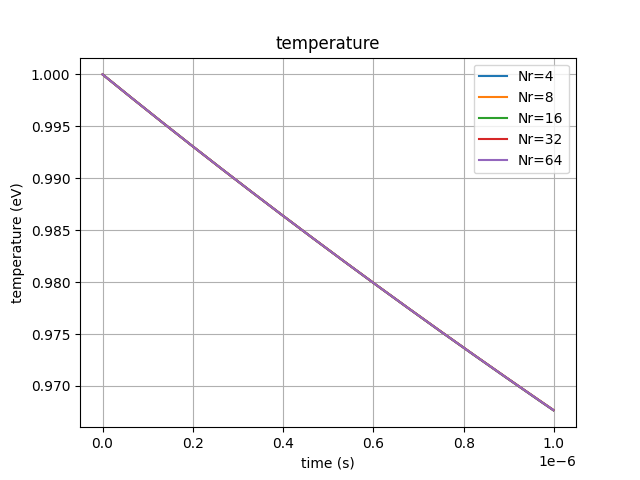
\includegraphics[width=0.48\textwidth]{g0_mw_temp.png}
				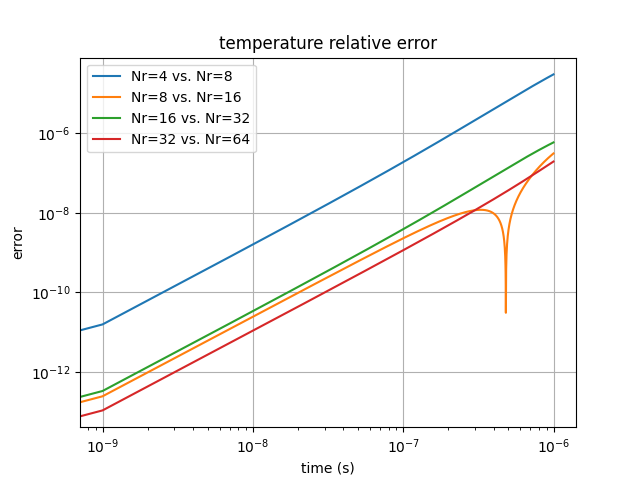
\includegraphics[width=0.48\textwidth]{g0_mw_temp_error.png}
			}
			\only<+>
			{
				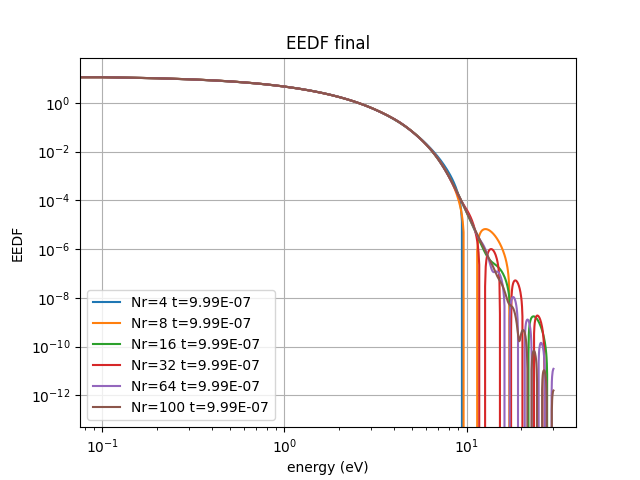
\includegraphics[width=0.48\textwidth]{g0_mw_eedf_final.png}
				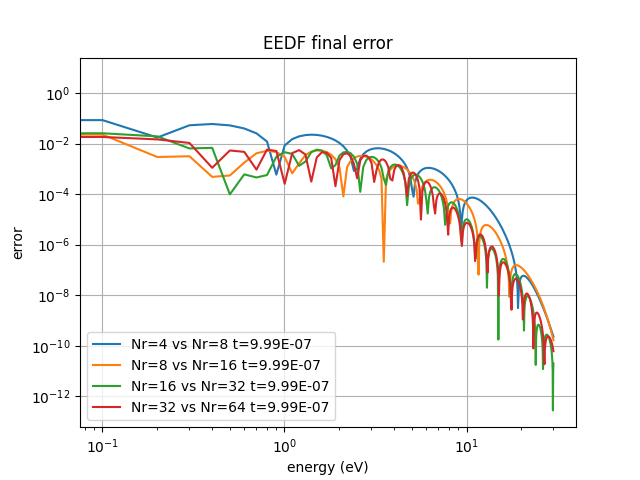
\includegraphics[width=0.48\textwidth]{g0_mw_eedf_final_error.png}
			}
		\end{figure}
	\end{frame}

	\begin{frame}
		\frametitle{Spectral convergence (Maxwell polynomials)}
		\begin{columns}
			\begin{column}{0.48\textwidth}
				\begin{itemize}
					\item Convergence of $f(v) = M(v) h(v)$,  $\rightarrow$ $\norm{f_{m}- f_{n}} \leq \norm{M(v)} \norm{h_m-h_n}$
					\item Tails of the correction term should decay with increasing $N_r$ polynomials.
					\item Reason ? \textcolor{orange}{We don't know yet.}
					\begin{itemize}
						\item May be we need more $N_r$ (Computation of Maxwell poly becomes unstable)
						\item Experimental cross-section data is not smooth. 
						\item Quadrature issues.
					\end{itemize}
				\end{itemize}
			\end{column}
			\begin{column}{0.48\textwidth}
				\begin{figure}
					\centering
					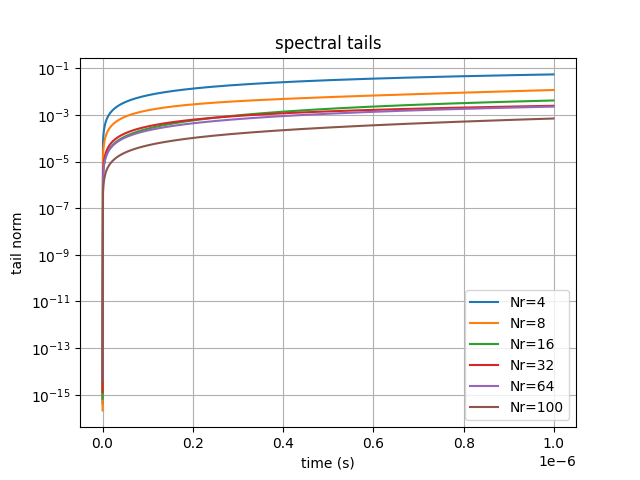
\includegraphics[width=\textwidth]{g0_mw_tails.png}
				\end{figure}
			\end{column}
		\end{columns}
	\end{frame}


	\begin{frame}
		\frametitle{G0 convergence with constant cross-section}
		\begin{figure}
			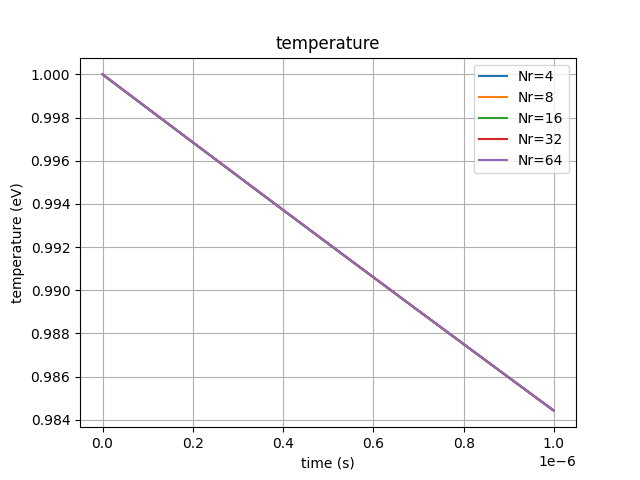
\includegraphics[width=0.48\textwidth]{g0_mw_m0_temp.png}
			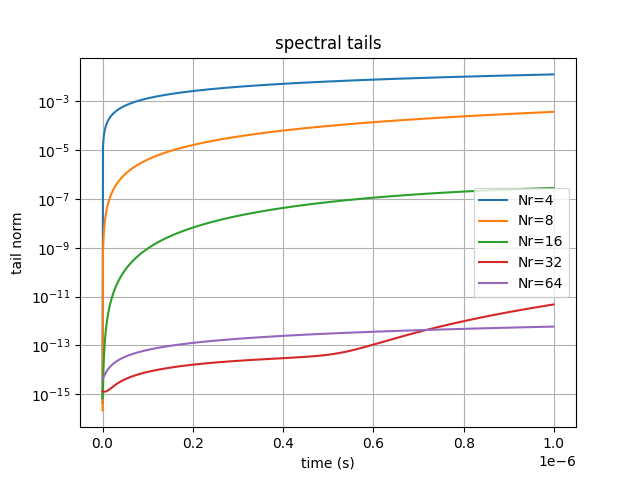
\includegraphics[width=0.48\textwidth]{g0_mw_m0_tails.png}
		\end{figure}
	\end{frame}


	\begin{frame}
		\frametitle{G0 convergence with linear cross-section}
		\begin{figure}
			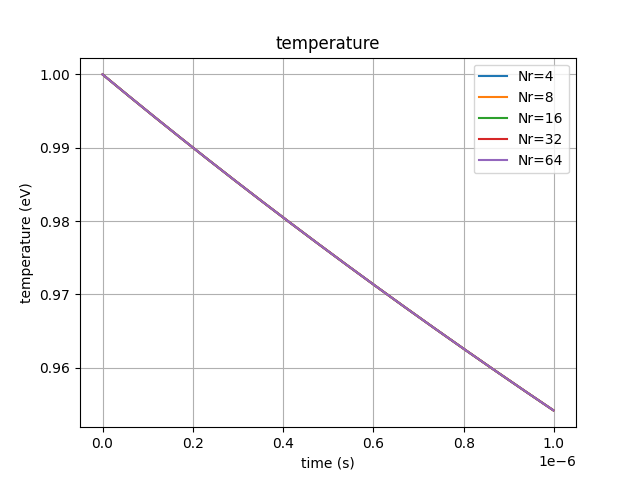
\includegraphics[width=0.48\textwidth]{g0_mw_m1_temp.png}
			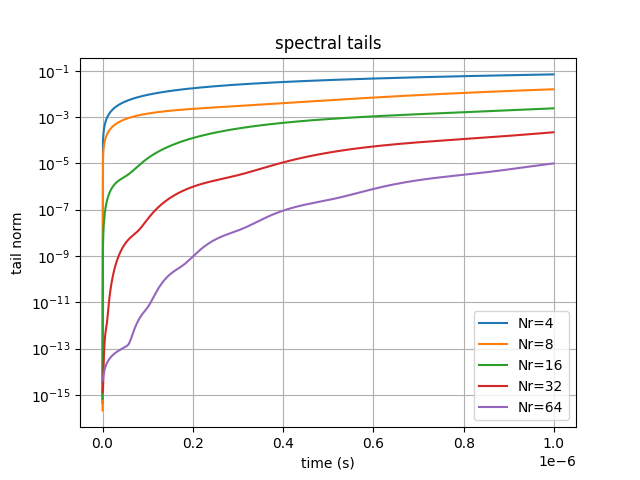
\includegraphics[width=0.48\textwidth]{g0_mw_m1_tails.png}
		\end{figure}
	\end{frame}
	
	\begin{frame}
		\frametitle{G0 : $e + Ar \rightarrow e + Ar$ (BSplines)}
		\begin{figure}
			\only<+>
			{
				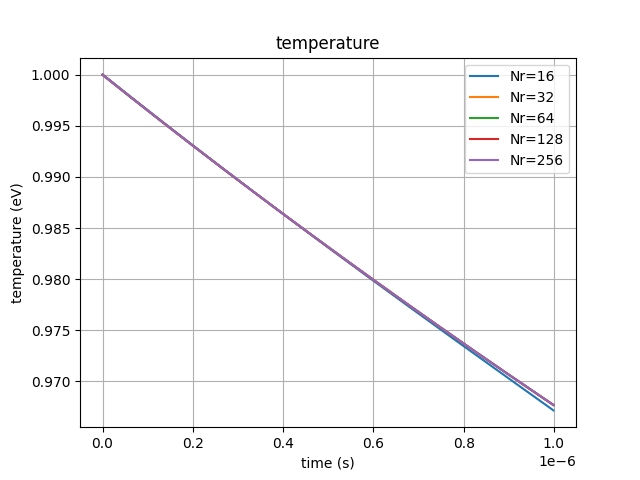
\includegraphics[width=0.48\textwidth]{g0_bs_temp.png}
				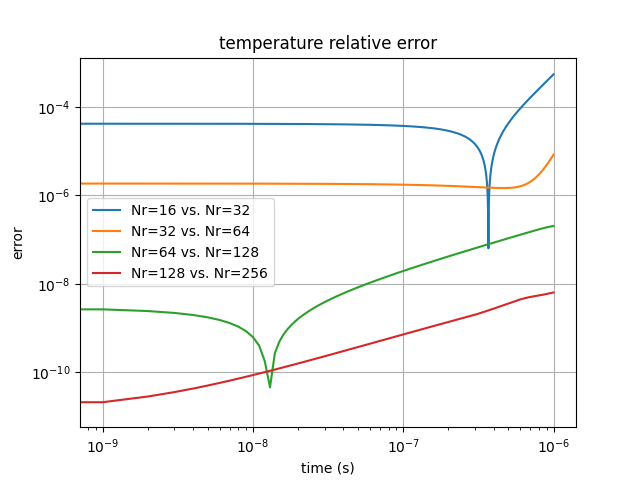
\includegraphics[width=0.48\textwidth]{g0_bs_temp_error.png}
			}
			\only<+>
			{
				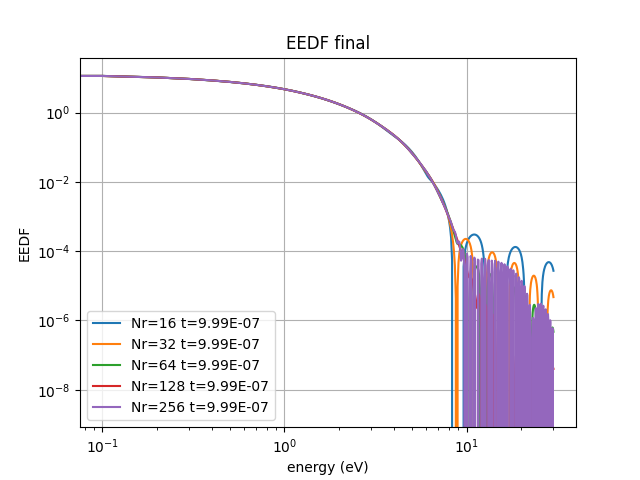
\includegraphics[width=0.48\textwidth]{g0_bs_eedf_final.png}
				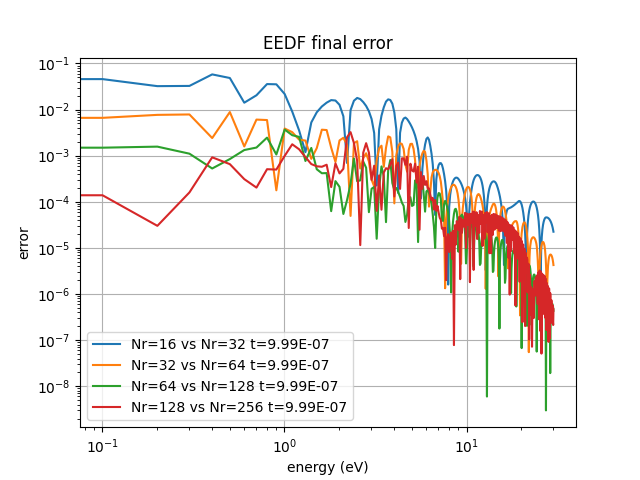
\includegraphics[width=0.48\textwidth]{g0_bs_eedf_final_error.png}
			}
		\end{figure}
	\end{frame}

	\begin{frame}
		\frametitle{Maxwell Vs. Bsplines : Elastic collisions (G0)}
		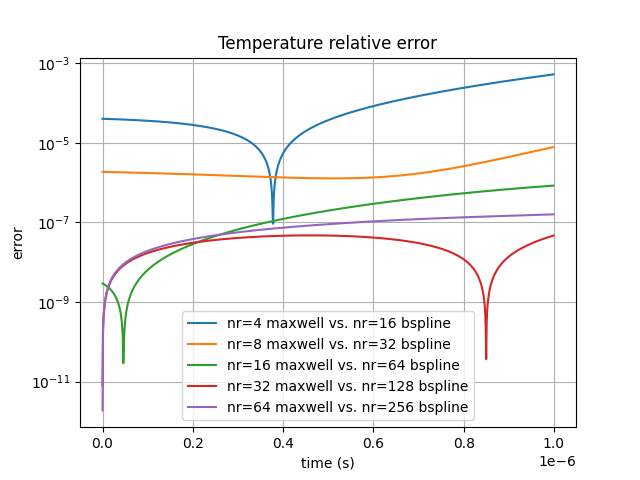
\includegraphics[width=0.48\textwidth]{g0_mw_bs_temp_error.png}
		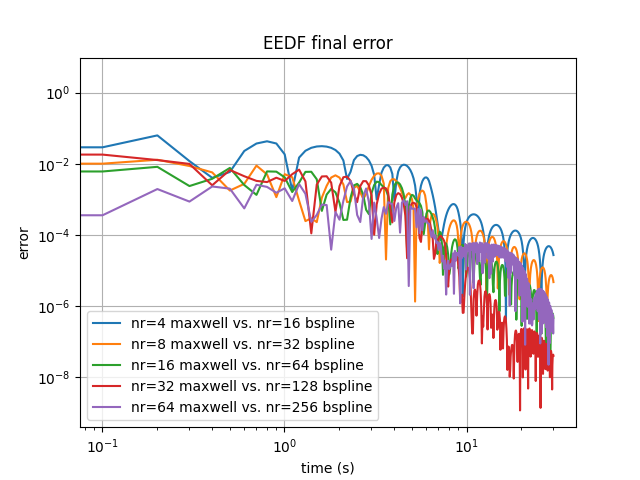
\includegraphics[width=0.48\textwidth]{g0_mw_bs_eedf_final_error.png}
	\end{frame}


	\begin{frame}
		\frametitle{Elastic with ionization (G0+G2)(Maxwell polynomials)}
		\begin{itemize}
			\item Quasi-neutrality enforces (problem becomes non-linear), $n_i=n_e$, $\partial_t f = n_0 C_{G0}(f) + n_i C_{G2}(f)$
			\item RK45 used for each linearized solve. 
		\end{itemize}
		\begin{figure}
			\only<+>
			{
				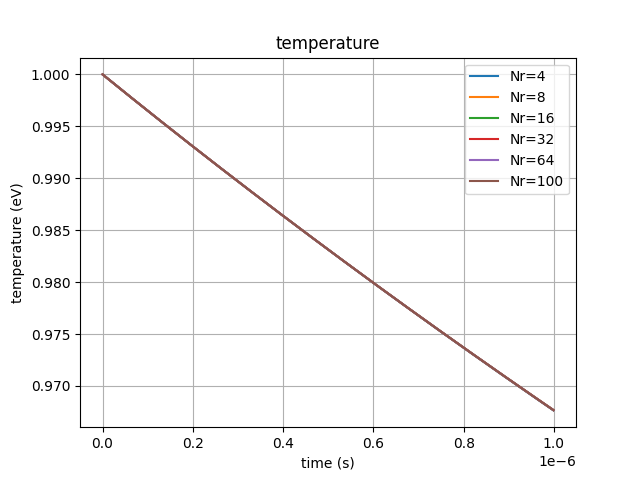
\includegraphics[width=0.48\textwidth]{g02_mw_temp.png}
				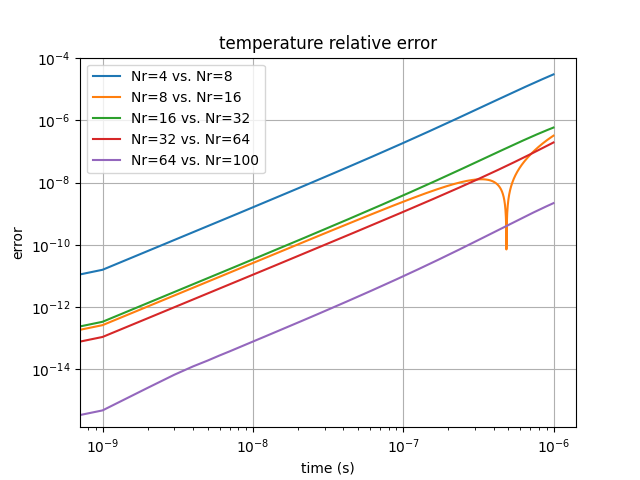
\includegraphics[width=0.48\textwidth]{g02_mw_temp_error.png}
			}
			\only<+>
			{
				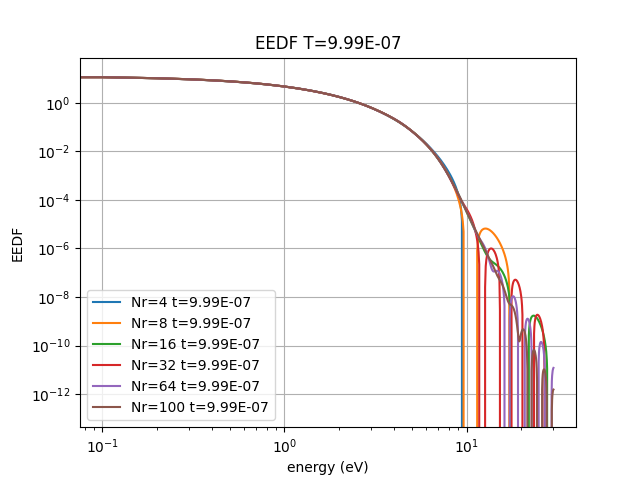
\includegraphics[width=0.48\textwidth]{g02_mw_eedf_final.png}
				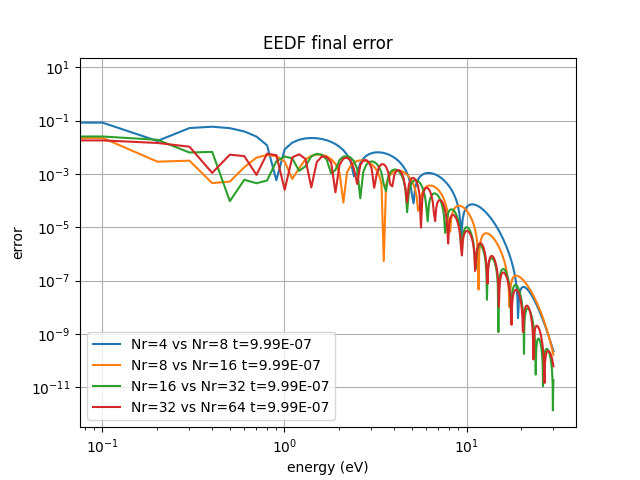
\includegraphics[width=0.48\textwidth]{g02_mw_eedf_final_error.png}
			}
			\only<+>
			{
				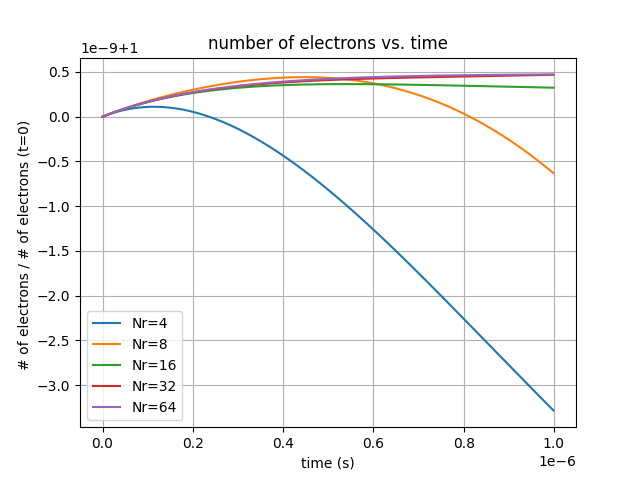
\includegraphics[width=0.48\textwidth]{g02_mw_mass.png}
			}
		\end{figure}
	\end{frame}


	\begin{frame}
		\frametitle{Projection operator}
		\begin{columns}
			\begin{column}{0.45\textwidth}
				\begin{itemize}
					\item All experiments are performed with a fixed Maxwellian, for specified temperature $T$. 
					\item Expansion of a $f_{T^\prime}$ for a given temperature $T\neq T^{\prime}$ $\rightarrow$ Large $N_r$. 
					\item One approach : Re-project and recompute the collision operators, when temperature changes. 
					\begin{itemize}
						\item computationally expensive. 
						\item introduce noise in the tails of the correction term. 
					\end{itemize}
					\item $M_{ij} = \frac{n}{\sqrt{\pi}^{3}}  \int_{R^3}  \exp(-v_\alpha^2) P_i (v_\alpha (1 + \frac{\epsilon}{\beta})) P_j(v_\alpha) \frac{dv}{\alpha}$
				\end{itemize} 
			\end{column}	
			\begin{column}{0.6\textwidth}
				\begin{figure}
					\only<+>
					{
						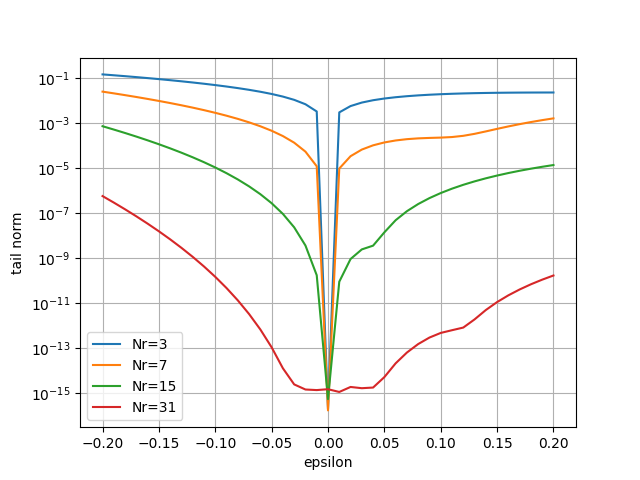
\includegraphics[width=0.8\textwidth]{../fig/basis_1ev_tail.png}
					}
					\only<+>
					{
						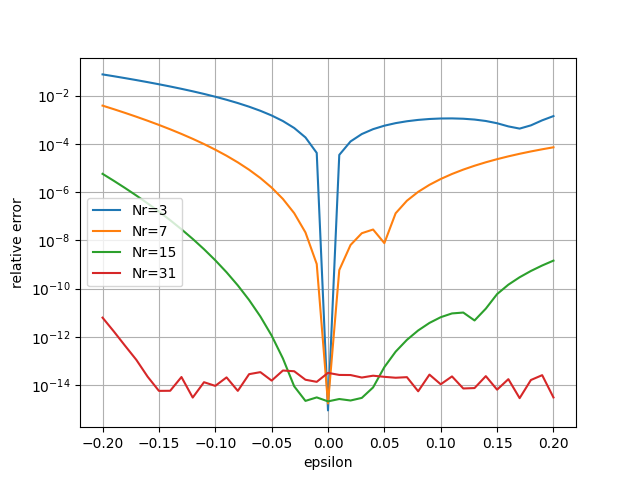
\includegraphics[width=0.8\textwidth]{../fig/basis_1ev_grid.png}
					}
					
				\end{figure}	
			\end{column}
		\end{columns}
	\end{frame}
	
	\begin{frame}{Current progress}
		\begin{itemize}
			\item Understand the Boltzmann collision operator with Jacobian for the collisions and how that relate to the weak form. 
			\item Derivation and numerically computation of Maxwell polynomials, associated quadrature. 
			\item \texttt{Python} based code for solving collission operator. 
			\item Integration with \texttt{LXCAT} cross-section data, for elastic, ionization and excitation reactions. 
			\item Supports Maxwell and BSplines for radial direction, other radial polynomials can be added if needed. 
			\item Tensoized version of the collision operator, (enables efficient GPU computations i.e., $\texttt{numpy} \rightarrow \texttt{cupy}$)
			\item Re-projection with efficient recomputation of the collision operator. 
		\end{itemize}
	\end{frame}

	\begin{frame}
		\frametitle{Conclusions and future work}
		\begin{itemize}
			\item Maxwell polynomials with experimental cross-section data, low convergence rate. 
			\item Dealing with smoothness issues, discontinuities in experimental cross section data. 
			\item Develop error metrics, when to perform re-projections, (only needed when operate in large temperature range.) , and numerical issues associated.
			\item Move on to single GPU implementation.
		\end{itemize}
		\pause
		\begin{center}
			\Large Questions ? \\
			\Large Thank You. 
		\end{center}
	\end{frame}


\end{document}
